\documentclass[11pt,a4paper]{article}

% ============================================
% PACKAGES
% ============================================
\usepackage[utf8]{inputenc}
\usepackage[T1]{fontenc}
\usepackage{graphicx}
\usepackage{longtable,booktabs,array}
\usepackage{multirow}
\usepackage{geometry}
\usepackage{hyperref}
\usepackage{titlesec}
\usepackage{fancyhdr}
\usepackage{xcolor}
\usepackage{float}
\usepackage{caption}
\usepackage{subcaption}
\usepackage{tocloft}
\usepackage{setspace}
\usepackage{amsmath}
\usepackage{amssymb}
\usepackage{booktabs}
\usepackage{array}
\usepackage{multirow}
\usepackage{enumitem}
\usepackage{parskip}
\usepackage{wrapfig}
\usepackage{multicol}
\usepackage{tikz}
\usepackage{pgfplots}
\usepackage{tcolorbox}
\usepackage{fontawesome5}
\usepackage{pifont}
\usepackage{epigraph}
\usepackage{lettrine}
\usepackage{microtype}
\usepackage{lipsum}

\pgfplotsset{compat=1.18}
\usetikzlibrary{shapes.geometric, arrows, positioning, calc, decorations.pathmorphing}

% ============================================
% PAGE GEOMETRY
% ============================================
\geometry{
    a4paper,
    left=18mm,
    right=18mm,
    top=18mm,
    bottom=18mm
}

% ============================================
% COLORS - COSMIC THEME
% ============================================
\definecolor{linkblue}{RGB}{0, 100, 180}
\definecolor{cosmicpurple}{RGB}{75, 0, 130}
\definecolor{nebulapink}{RGB}{199, 21, 133}
\definecolor{stargold}{RGB}{255, 193, 37}
\definecolor{deepspace}{RGB}{25, 25, 50}
\definecolor{darkgray}{RGB}{64, 64, 64}
\definecolor{lightcosmic}{RGB}{240, 240, 255}

% ============================================
% TCOLORBOX STYLES
% ============================================
\tcbuselibrary{skins,breakable}

% Fun Fact Box
\newtcolorbox{funfactbox}[1][]{
    enhanced,
    breakable,
    colback=lightcosmic,
    colframe=cosmicpurple,
    arc=3mm,
    boxrule=1.5pt,
    left=10pt,
    right=10pt,
    top=8pt,
    bottom=8pt,
    fonttitle=\bfseries,
    title={\faLightbulb\ \ Did You Know?},
    #1
}

% Scientist Biography Box
\newtcolorbox{scientistbox}[2][]{
    enhanced,
    breakable,
    colback=white,
    colframe=stargold,
    arc=2mm,
    boxrule=1.2pt,
    left=10pt,
    right=10pt,
    top=8pt,
    bottom=8pt,
    fonttitle=\bfseries\color{darkgray},
    title={\faUserGraduate\ \ #2},
    #1
}

% Key Concept Box
\newtcolorbox{conceptbox}[2][]{
    enhanced,
    breakable,
    colback=white,
    colframe=nebulapink,
    arc=2mm,
    boxrule=1.2pt,
    left=10pt,
    right=10pt,
    top=8pt,
    bottom=8pt,
    fonttitle=\bfseries,
    title={\faAtom\ \ #2},
    #1
}

% Equation Highlight Box
\newtcolorbox{equationbox}[1][]{
    enhanced,
    colback=lightcosmic,
    colframe=deepspace,
    arc=1mm,
    boxrule=0.8pt,
    left=5pt,
    right=5pt,
    top=5pt,
    bottom=5pt,
    #1
}

% Timeline Event Box
\newtcolorbox{timelinebox}[2][]{
    enhanced,
    colback=white,
    colframe=linkblue,
    arc=2mm,
    boxrule=1pt,
    left=8pt,
    right=8pt,
    top=5pt,
    bottom=5pt,
    fonttitle=\bfseries\small,
    title={#2},
    #1
}

% ============================================
% HYPERREF SETUP
% ============================================
\hypersetup{
    colorlinks=true,
    linkcolor=cosmicpurple,
    filecolor=black,
    urlcolor=linkblue,
    citecolor=nebulapink,
    pdftitle={The Invisible Universe - Comprehensive Project Report},
    pdfauthor={Team BomBSquad},
    pdfsubject={Dark Matter, Black Holes, Big Bang Theory},
    pdfkeywords={cosmology, dark matter, black holes, Big Bang, astrophysics}
}

% ============================================
% HEADER AND FOOTER
% ============================================
\pagestyle{fancy}
\fancyhf{}
\fancyhead[L]{\small\textit{The Invisible Universe}}
\fancyhead[R]{\small\textit{Team BomBSquad}}
\fancyfoot[C]{\thepage}
\renewcommand{\headrulewidth}{0.4pt}
\renewcommand{\footrulewidth}{0.4pt}

% ============================================
% TITLE FORMATTING
% ============================================
\titleformat{\section}
{\normalfont\Large\bfseries\color{cosmicpurple}}
{\thesection}{1em}{}[\titlerule]
\titlespacing*{\section}{0pt}{1.5ex plus 0.3ex minus 0.2ex}{1ex plus 0.2ex}

\titleformat{\subsection}
{\normalfont\large\bfseries\color{deepspace}}
{\thesubsection}{1em}{}
\titlespacing*{\subsection}{0pt}{1ex plus 0.3ex minus 0.2ex}{0.8ex plus 0.2ex}

\titleformat{\subsubsection}
{\normalfont\normalsize\bfseries\color{darkgray}}
{\thesubsubsection}{1em}{}
\titlespacing*{\subsubsection}{0pt}{0.8ex plus 0.2ex minus 0.1ex}{0.5ex plus 0.1ex}

% ============================================
% TABLE OF CONTENTS FORMATTING
% ============================================
\renewcommand{\cftsecleader}{\cftdotfill{\cftdotsep}}
\setlength{\cftbeforesecskip}{3pt}

% ============================================
% SPACING
% ============================================
\setlength{\parskip}{0.25em}
\setlength{\parindent}{0pt}
\setstretch{1.12}

% ============================================
% CUSTOM COMMANDS
% ============================================
\newcommand{\msun}{M_\odot}
\newcommand{\lsun}{L_\odot}
\newcommand{\kms}{\text{km/s}}
\newcommand{\mpc}{\text{Mpc}}
\newcommand{\kpc}{\text{kpc}}
\newcommand{\lyr}{\text{ly}}
\newcommand{\gev}{\text{GeV}}
\newcommand{\ev}{\text{eV}}
\newcommand{\kelvin}{\text{K}}

% Checkmark and cross
\newcommand{\cmark}{\ding{51}}
\newcommand{\xmark}{\ding{55}}

% ============================================
% DOCUMENT START
% ============================================
\begin{document}


% ============================================
% TABLE OF CONTENTS - PAGE 1
% ============================================
\pagenumbering{arabic}
\setcounter{page}{1}

\tableofcontents
\thispagestyle{fancy}

\newpage

% ============================================
% LIST OF FIGURES AND TABLES - PAGE 2
% ============================================
\listoffigures
\listoftables

\newpage

% ============================================
% SECTION 1: INTRODUCTION
% ============================================
\section{Introduction}
\label{sec:introduction}

\lettrine[lines=3, loversize=0.1, nindent=0.5em]{W}{hen} we gaze upon the night sky, we witness merely the tip of a cosmic iceberg. The glittering tapestry of stars, galaxies, and nebulae that has inspired humanity for millennia represents an astonishingly small fraction of what actually exists. Modern astrophysics has revealed a startling truth: approximately 95\% of all matter and energy in the cosmos remains completely invisible to our most sophisticated instruments.

This project, \textbf{``The Invisible Universe,''} embarks on a comprehensive investigation of this hidden cosmos, focusing on three fundamental aspects that define our understanding of the universe's structure and evolution.

\subsection{The Cosmic Census: What Is the Universe Made Of?}

The European Space Agency's Planck satellite mission (2009--2013) provided humanity's most precise measurement of the universe's composition. The results challenge our intuitive understanding of reality:

\begin{figure}[H]
    \centering
    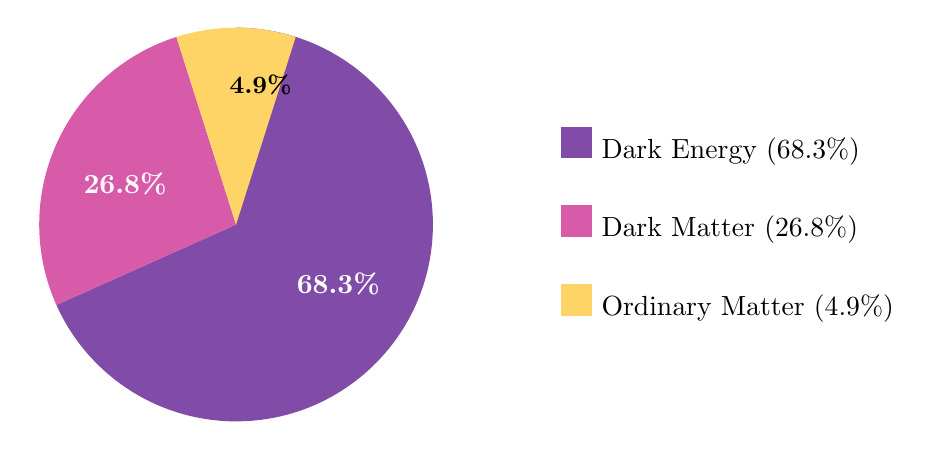
\begin{tikzpicture}
        % Manual pie chart
        \def\radius{2.5}
        % Dark Energy: 68.3% = 245.88 degrees
        \fill[cosmicpurple!70] (0,0) -- (90:\radius) arc (90:-155.88:\radius) -- cycle;
        % Dark Matter: 26.8% = 96.48 degrees
        \fill[nebulapink!70] (0,0) -- (-155.88:\radius) arc (-155.88:-252.36:\radius) -- cycle;
        % Ordinary Matter: 4.9% = 17.64 degrees
        \fill[stargold!70] (0,0) -- (-252.36:\radius) arc (-252.36:-270:\radius) -- cycle;
        \fill[stargold!70] (0,0) -- (90:\radius) arc (90:72.36:\radius) -- cycle;

        % Labels
        \node[white, font=\bfseries] at (-30:1.5) {68.3\%};
        \node[white, font=\bfseries] at (-200:1.5) {26.8\%};
        \node[font=\bfseries\small] at (80:1.8) {4.9\%};

        % Legend
        \node[right] at (4, 1) {\tikz\fill[cosmicpurple!70] (0,0) rectangle (0.4,0.4); Dark Energy (68.3\%)};
        \node[right] at (4, 0) {\tikz\fill[nebulapink!70] (0,0) rectangle (0.4,0.4); Dark Matter (26.8\%)};
        \node[right] at (4, -1) {\tikz\fill[stargold!70] (0,0) rectangle (0.4,0.4); Ordinary Matter (4.9\%)};
    \end{tikzpicture}
    \caption{Composition of the universe according to Planck satellite measurements (2018).}
    \label{fig:universe_composition}
\end{figure}

\begin{itemize}[noitemsep]
    \item \textbf{68.3\% Dark Energy:} A mysterious repulsive force causing the universe's expansion to accelerate. Discovered in 1998 through observations of Type Ia supernovae by the Supernova Cosmology Project and High-Z Supernova Search Team, earning Perlmutter, Schmidt, and Riess the 2011 Nobel Prize in Physics. Its physical nature remains unknown.

    \item \textbf{26.8\% Dark Matter:} Invisible matter detectable only through its gravitational influence. It does not emit, absorb, or reflect electromagnetic radiation of any wavelength. First proposed by Fritz Zwicky in 1933, its existence is now confirmed through multiple independent observations.

    \item \textbf{4.9\% Baryonic (Ordinary) Matter:} Everything we can see and touch---all stars, planets, gas clouds, dust, and living organisms. This includes every atom in your body, every star in every galaxy, and all the interstellar gas and dust throughout the cosmos.
\end{itemize}

\subsection{The Three Pillars of the Invisible Universe}

This report investigates three interconnected phenomena that together reveal the hidden architecture of the cosmos:

\begin{conceptbox}{The Three Pillars}
\begin{enumerate}[noitemsep]
    \item \textbf{Dark Matter} --- The invisible scaffolding upon which all cosmic structure is built
    \item \textbf{Black Holes} --- Regions where gravity has completely conquered light itself
    \item \textbf{The Big Bang} --- The origin event from which space, time, and all matter emerged
\end{enumerate}
\end{conceptbox}

\subsection{Project Objectives}

This comprehensive investigation aims to:

\begin{enumerate}[noitemsep]
    \item Present and analyze multiple independent lines of evidence confirming dark matter's existence
    \item Explain black hole physics from theoretical foundations to recent observational breakthroughs
    \item Describe the Big Bang model and trace cosmic evolution from $10^{-43}$ seconds to the present
    \item Examine galaxy clusters as cosmic laboratories for studying dark matter
    \item Explore gravitational wave astronomy as a new window on the universe
    \item Showcase scientific imagery from NASA, ESA, and international collaborations
    \item Discuss dark energy and the accelerating expansion of the universe
    \item Survey ongoing and future experiments designed to detect dark matter particles
    \item Create an educational resource combining rigorous science with accessibility
\end{enumerate}

\subsection{Observational Foundations}

Our analysis draws upon data from humanity's most advanced astronomical instruments:

\begin{table}[H]
\centering
\caption{Primary data sources for this investigation.}
\label{tab:data_sources}
\small
\begin{tabular}{|l|l|l|l|}
\hline
\textbf{Observatory} & \textbf{Type} & \textbf{Key Capability} & \textbf{Launch} \\
\hline
Hubble Space Telescope & Optical/UV/IR & 2.4m mirror, 0.05'' resolution & 1990 \\
Chandra X-ray Observatory & X-ray & 0.5'' resolution, 0.1--10 keV & 1999 \\
Planck Satellite & Microwave & $\mu$K CMB precision & 2009 \\
Event Horizon Telescope & Radio VLBI & $\mu$as resolution & 2017 \\
LIGO/Virgo & Gravitational Wave & Strain $\sim 10^{-23}$ & 2015 \\
James Webb Space Telescope & Infrared & 6.5m mirror, $z > 13$ & 2021 \\
\hline
\end{tabular}
\end{table}

\newpage

% ============================================
% SECTION 2: HISTORICAL TIMELINE
% ============================================
\section{Historical Timeline of Discovery}
\label{sec:history}

The journey to understanding the invisible universe spans over a century of scientific investigation, marked by theoretical breakthroughs and observational surprises. Moreover, this remarkable progression demonstrates how fundamental physics and advanced technology have collaboratively transformed our comprehension of cosmic phenomena. Consequently, each discovery has built upon previous findings, creating an interconnected web of knowledge that continues to expand our understanding of the universe's hidden architecture.

\subsection{Key Milestones in Cosmology}

\begin{table}[H]
\centering
\caption{Timeline of major discoveries in understanding the invisible universe.}
\label{tab:history_timeline}
\small
\begin{tabular}{|l|l|p{9cm}|}
\hline
\textbf{Year} & \textbf{Discovery} & \textbf{Significance} \\
\hline
1915 & General Relativity & Einstein describes gravity as spacetime curvature \\
1916 & Schwarzschild Solution & First black hole solution: $r_s = 2GM/c^2$ \\
1929 & Hubble Expansion & Universe is expanding: $v = H_0 d$ \\
1933 & Dark Matter & Zwicky finds ``missing mass'' in Coma Cluster \\
1965 & CMB Discovery & Penzias \& Wilson detect Big Bang afterglow \\
1970s & Rotation Curves & Rubin \& Ford confirm flat galaxy rotation curves \\
1998 & Dark Energy & Supernovae reveal accelerating expansion \\
2006 & Bullet Cluster & Direct proof of dark matter as real substance \\
2015 & Gravitational Waves & LIGO detects merging black holes \\
2019 & M87* Image & EHT captures first black hole shadow \\
2022 & Sgr A* Image & EHT images Milky Way's central black hole \\
\hline
\end{tabular}
\end{table}

\begin{scientistbox}{Key Pioneers}
\textbf{Albert Einstein} (1879--1955): General relativity; $G_{\mu\nu} + \Lambda g_{\mu\nu} = \frac{8\pi G}{c^4} T_{\mu\nu}$. \textbf{Fritz Zwicky} (1898--1974): First proposed dark matter from cluster dynamics. \textbf{Vera Rubin} (1928--2016): Galaxy rotation curves proving dark matter halos. \textbf{Stephen Hawking} (1942--2018): Black hole radiation and quantum gravity.
\end{scientistbox}

\newpage

% ============================================
% SECTION 3: BLACK HOLES
% ============================================
\section{Black Holes: Where Gravity Conquers Light}
\label{sec:blackholes}

\lettrine[lines=3, loversize=0.1, nindent=0.5em]{B}{lack} holes represent nature's most extreme objects---regions of spacetime where gravitational attraction is so intense that nothing, not even light traveling at 299,792,458 meters per second, can escape once past a boundary called the event horizon. Furthermore, these extraordinary cosmic entities challenge our fundamental understanding of physics, as they exist at the intersection of general relativity and quantum mechanics. Nevertheless, despite their inherently invisible nature, astronomers have developed increasingly sophisticated methods to detect and study these fascinating objects through their gravitational influence on surrounding matter and spacetime.

\subsection{Theoretical Foundations}

\subsubsection{The Schwarzschild Metric}

The spacetime geometry around a non-rotating, uncharged black hole is described by Karl Schwarzschild's 1916 solution to Einstein's field equations. Remarkably, Schwarzschild derived this solution while serving on the Russian front during World War I, and it remains one of the most important exact solutions in general relativity. Accordingly, this mathematical framework provides the foundation for understanding how mass curves spacetime in the most extreme gravitational environments:

\begin{equationbox}
\begin{equation}
ds^2 = -\left(1 - \frac{r_s}{r}\right)c^2 dt^2 + \left(1 - \frac{r_s}{r}\right)^{-1} dr^2 + r^2(d\theta^2 + \sin^2\theta \, d\phi^2)
\label{eq:schwarzschild}
\end{equation}
\end{equationbox}

where the \textbf{Schwarzschild radius} is:

\begin{equationbox}
\begin{equation}
r_s = \frac{2GM}{c^2}
\label{eq:schwarzschild_radius}
\end{equation}
\end{equationbox}

\begin{itemize}[noitemsep]
    \item $G = 6.674 \times 10^{-11}$ m$^3$ kg$^{-1}$ s$^{-2}$ (gravitational constant)
    \item $M$ = mass of the black hole
    \item $c = 2.998 \times 10^8$ m/s (speed of light)
\end{itemize}

\subsubsection{Physical Interpretation}

At $r = r_s$, the metric coefficient $(1 - r_s/r)$ becomes zero, creating a coordinate singularity---the \textbf{event horizon}. Key properties:

\begin{itemize}[noitemsep]
    \item \textbf{One-way membrane:} Information and matter can fall in but never escape
    \item \textbf{Time dilation:} Clocks slow dramatically near the horizon; to a distant observer, infalling objects appear to freeze at $r = r_s$
    \item \textbf{Gravitational redshift:} Light escaping from near the horizon loses energy, becoming increasingly redshifted
    \item \textbf{Tidal forces:} Near the singularity at $r = 0$, tidal stretching (``spaghettification'') destroys any object
\end{itemize}

\subsubsection{Calculated Examples}

\begin{table}[H]
\centering
\caption{Schwarzschild radii for various objects.}
\label{tab:schwarzschild}
\begin{tabular}{|l|c|c|c|}
\hline
\textbf{Object} & \textbf{Mass (kg)} & \textbf{$r_s$} & \textbf{Comparison} \\
\hline
Earth & $5.97 \times 10^{24}$ & 8.87 mm & Marble \\
Sun & $1.99 \times 10^{30}$ & 2.95 km & Small town \\
Sagittarius A* & $8.2 \times 10^{36}$ & 1.2 $\times 10^{7}$ km & 17 $\times$ Sun's radius \\
M87* & $1.3 \times 10^{40}$ & $1.9 \times 10^{10}$ km & 3 $\times$ Pluto's orbit \\
\hline
\end{tabular}
\end{table}

\subsection{Rotating Black Holes: The Kerr Solution}

Most astrophysical black holes rotate, often quite rapidly, as a natural consequence of angular momentum conservation during their formation process. Therefore, Roy Kerr's 1963 solution, which describes rotating black holes, represents a more physically realistic model than Schwarzschild's non-rotating case. Specifically, this solution introduces several fascinating new phenomena that have significant implications for both theoretical physics and observational astronomy:

\begin{equationbox}
\begin{equation}
ds^2 = -\left(1 - \frac{r_s r}{\Sigma}\right)c^2 dt^2 - \frac{2r_s r a \sin^2\theta}{\Sigma} c \, dt \, d\phi + \frac{\Sigma}{\Delta} dr^2 + \Sigma \, d\theta^2
\end{equation}
\end{equationbox}

where $a = J/Mc$ is the spin parameter, $\Sigma = r^2 + a^2\cos^2\theta$, and $\Delta = r^2 - r_s r + a^2$.

\textbf{Key features of Kerr black holes:}

\begin{itemize}[noitemsep]
    \item \textbf{Ergosphere:} A region outside the event horizon where spacetime is dragged so strongly that nothing can remain stationary
    \item \textbf{Frame dragging:} Spacetime itself is twisted by the rotation (Lense-Thirring effect)
    \item \textbf{Penrose process:} Energy can theoretically be extracted from a rotating black hole
    \item \textbf{Maximum spin:} $a \leq GM/c^2$ (extremal limit)
\end{itemize}

\subsection{Classification by Mass}

Black holes span an enormous range of masses, from a few solar masses to billions:

\begin{table}[H]
\centering
\caption{Classification of black holes by mass.}
\label{tab:bh_classification}
\begin{tabular}{|l|l|l|l|}
\hline
\textbf{Type} & \textbf{Mass Range} & \textbf{Formation Mechanism} & \textbf{Examples} \\
\hline
Stellar & 5--100 $\msun$ & Core collapse of massive stars & Cygnus X-1 \\
Intermediate & $10^2$--$10^5$ $\msun$ & Stellar mergers, runaway collisions & HLX-1 \\
Supermassive & $10^6$--$10^{10}$ $\msun$ & Hierarchical growth, direct collapse & M87*, Sgr A* \\
Primordial & $10^{-8}$--$10^5$ $\msun$ & Early universe density fluctuations & Hypothetical \\
\hline
\end{tabular}
\end{table}

\subsection{Hawking Radiation: Black Holes Aren't Forever}

In 1974, Stephen Hawking demonstrated one of the most profound connections between quantum mechanics and general relativity by showing that black holes aren't perfectly black---instead, they emit thermal radiation due to quantum effects near the event horizon. Consequently, this groundbreaking theoretical discovery, now known as Hawking radiation, implies that black holes gradually lose mass over extremely long timescales and will eventually evaporate completely. Furthermore, this phenomenon raises deep questions about information conservation in physics, leading to what is now called the ``black hole information paradox,'' which remains an active area of research in theoretical physics:

\begin{equationbox}
\begin{equation}
T_H = \frac{\hbar c^3}{8\pi G M k_B} \approx \frac{6.2 \times 10^{-8}}{M/\msun} \text{ K}
\label{eq:hawking_temp}
\end{equation}
\end{equationbox}

\begin{itemize}[noitemsep]
    \item A stellar-mass black hole: $T_H \sim 10^{-8}$ K (undetectable)
    \item Black hole evaporation time: $t_{evap} \sim 10^{67} (M/\msun)^3$ years
\end{itemize}

\subsection{Observational Breakthroughs}

\subsubsection{Event Horizon Telescope: First Direct Image}

On April 10, 2019, humanity witnessed the first direct image of a black hole---M87* at the center of the giant elliptical galaxy Messier 87. This historic achievement represented the culmination of decades of technological development and international scientific collaboration. Moreover, the image confirmed key predictions of Einstein's general relativity in the strong-field regime and provided unprecedented insights into the physics of accretion disks and relativistic jets. Notably, this accomplishment required coordinating eight radio telescopes across four continents to effectively create an Earth-sized virtual telescope.

\begin{figure}[H]
    \centering
    \includegraphics[width=0.65\textwidth]{../images/scientific/blackhole_m87.jpg}
    \caption{First direct image of a black hole shadow---M87* captured by the Event Horizon Telescope, April 2019. The bright ring is synchrotron radiation from relativistic electrons; the dark center is the black hole's shadow.}
    \label{fig:m87}
\end{figure}

\textbf{Technical Achievement:}

\begin{table}[H]
\centering
\caption{Event Horizon Telescope observation parameters for M87*.}
\label{tab:eht_params}
\begin{tabular}{|l|l|}
\hline
\textbf{Parameter} & \textbf{Value} \\
\hline
Target Mass & $(6.5 \pm 0.7) \times 10^9$ $\msun$ \\
Distance & 54.8 million light-years (16.8 Mpc) \\
Angular Size & $42 \pm 3$ microarcseconds \\
Observation Wavelength & 1.3 mm (230 GHz) \\
Observation Dates & April 5--11, 2017 \\
Number of Telescopes & 8 (spanning 4 continents) \\
Effective Aperture & Earth-sized ($\sim$10,000 km baseline) \\
Angular Resolution & 20 microarcseconds \\
Data Volume & 5 petabytes \\
\hline
\end{tabular}
\end{table}

\subsubsection{Key Observational Milestones}

\begin{table}[H]
\centering
\caption{Timeline of black hole observation milestones.}
\label{tab:bh_timeline}
\begin{tabular}{|l|l|}
\hline
\textbf{Year} & \textbf{Milestone} \\
\hline
1971 & Cygnus X-1 identified as first strong black hole candidate \\
1994 & Hubble confirms supermassive black hole in M87 center \\
2002 & Stellar orbits reveal Sgr A* mass ($4 \times 10^6$ $\msun$) \\
2015 & LIGO detects gravitational waves from binary BH merger (GW150914) \\
2019 & Event Horizon Telescope images M87* shadow \\
2020 & Nobel Prize to Penrose, Genzel, and Ghez for BH research \\
2022 & EHT images Sagittarius A* (Milky Way's central BH) \\
\hline
\end{tabular}
\end{table}

\newpage

% ============================================
% SECTION 4: DARK MATTER
% ============================================
\section{Dark Matter: The Invisible Scaffolding}
\label{sec:darkmatter}

\lettrine[lines=3, loversize=0.1, nindent=0.5em]{D}{ark} matter constitutes approximately 85\% of all matter in the universe, yet its fundamental nature remains one of physics' greatest unsolved mysteries. We cannot see it, touch it, or detect it with any electromagnetic instrument---nevertheless, its gravitational fingerprints are unmistakably present throughout the cosmos. Furthermore, without dark matter, galaxies would not have formed, stars would not exist, and life as we know it would be impossible. Consequently, understanding this invisible substance represents one of the most important challenges in modern astrophysics and particle physics.

\subsection{Theoretical Framework}

Dark matter must satisfy several observational constraints:

\begin{itemize}[noitemsep]
    \item \textbf{Electrically neutral:} Does not interact with electromagnetic radiation
    \item \textbf{Collisionless:} Self-interaction cross-section $\sigma/m < 1$ cm$^2$/g
    \item \textbf{Cold:} Non-relativistic at the epoch of structure formation
    \item \textbf{Stable:} Lifetime $\tau \gg$ age of universe ($13.8 \times 10^9$ years)
    \item \textbf{Non-baryonic:} Cannot be made of protons and neutrons
\end{itemize}

\subsection{Evidence for Dark Matter}

\subsubsection{Evidence 1: Galaxy Rotation Curves}

According to Newtonian mechanics, the orbital velocity of stars in a galaxy should follow:

\begin{equationbox}
\begin{equation}
v(r) = \sqrt{\frac{GM(r)}{r}}
\label{eq:rotation}
\end{equation}
\end{equationbox}

Beyond the visible disk, where $M(r)$ should be approximately constant, we expect $v \propto r^{-1/2}$---a ``Keplerian decline.'' However, observations consistently show \textbf{flat rotation curves} extending far beyond the visible matter. Notably, Vera Rubin and Kent Ford first systematically documented this phenomenon in the 1970s, providing compelling evidence that galaxies must be embedded in massive halos of invisible matter. Accordingly, this discrepancy between theoretical predictions and observational data has become one of the strongest pieces of evidence supporting the existence of dark matter.

\begin{figure}[H]
    \centering
    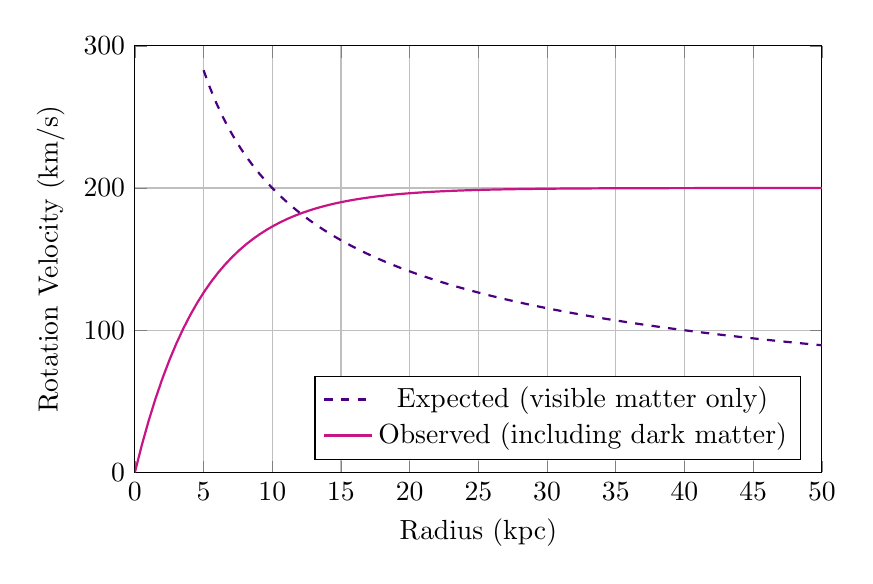
\begin{tikzpicture}
        \begin{axis}[
            width=0.85\textwidth,
            height=7cm,
            xlabel={Radius (kpc)},
            ylabel={Rotation Velocity (km/s)},
            xmin=0, xmax=50,
            ymin=0, ymax=300,
            legend pos=south east,
            grid=major
        ]
        % Expected (Keplerian)
        \addplot[domain=5:50, samples=100, dashed, thick, cosmicpurple] {200*sqrt(10/x)};
        \addlegendentry{Expected (visible matter only)}

        % Observed (flat)
        \addplot[domain=0:50, samples=100, thick, nebulapink] {200*(1 - exp(-x/5))};
        \addlegendentry{Observed (including dark matter)}

        \end{axis}
    \end{tikzpicture}
    \caption{Schematic galaxy rotation curve showing expected Keplerian decline vs. observed flat profile.}
    \label{fig:rotation_curve}
\end{figure}

This discrepancy requires 5--10 times more mass than visible matter can account for, which strongly suggests the presence of an unseen gravitational component surrounding every galaxy.

\subsubsection{Evidence 2: The Bullet Cluster (``Smoking Gun'')}

The Bullet Cluster (1E 0657-56) provides the most direct empirical proof of dark matter's existence as a distinct physical substance. Specifically, this remarkable cosmic collision has become known as the ``smoking gun'' for dark matter because it demonstrates the separation of gravitating mass from ordinary baryonic matter. Moreover, this observation effectively rules out modified gravity theories as alternatives to dark matter, since the gravitational lensing signal clearly traces the dark matter distribution rather than the visible gas.

\begin{figure}[H]
    \centering
    \begin{minipage}{0.48\textwidth}
        \centering
        \includegraphics[width=\textwidth]{../images/scientific/bullet_cluster_composite.jpg}
        \caption{Composite image: dark matter (blue, from lensing) separated from hot gas (pink, from X-rays).}
        \label{fig:bullet_composite}
    \end{minipage}\hfill
    \begin{minipage}{0.48\textwidth}
        \centering
        \includegraphics[width=\textwidth]{../images/scientific/bullet_cluster_dark_matter.png}
        \caption{Chandra X-ray image showing the shock front and gas distribution.}
        \label{fig:bullet_xray}
    \end{minipage}
\end{figure}

\textbf{The Collision Physics:}

Approximately 150 million years ago, a smaller galaxy cluster plowed through a larger one at $\sim$4,500 km/s (Mach 3). The components behaved differently:

\begin{table}[H]
\centering
\caption{Behavior of different components during the Bullet Cluster collision.}
\label{tab:bullet_components}
\begin{tabular}{|l|c|l|l|}
\hline
\textbf{Component} & \textbf{Mass Fraction} & \textbf{Interaction} & \textbf{Behavior} \\
\hline
Dark Matter & 85\% & Collisionless (gravity only) & Passed through unimpeded \\
Hot Gas (ICM) & 12\% & Electromagnetic drag & Slowed, shocked, heated \\
Galaxies (Stars) & 3\% & Weak (stars rarely collide) & Passed through with tides \\
\hline
\end{tabular}
\end{table}

The key observation: \textbf{gravitational lensing maps show the mass concentration offset from the X-ray gas by $\sim$720 kpc}. This is impossible if gravity follows matter or if dark matter doesn't exist.

\subsubsection{Evidence 3: Gravitational Lensing}

Mass bends spacetime, causing light to follow curved paths. The deflection angle for a point mass is:

\begin{equationbox}
\begin{equation}
\alpha = \frac{4GM}{c^2 b}
\label{eq:deflection}
\end{equation}
\end{equationbox}

where $b$ is the impact parameter (closest approach distance).

\begin{figure}[H]
    \centering
    \begin{minipage}{0.48\textwidth}
        \centering
        \includegraphics[width=\textwidth]{../images/scientific/lensing_diagram_dark.png}
        \caption{Gravitational lensing geometry showing light bending around a massive object.}
        \label{fig:lensing_diagram}
    \end{minipage}\hfill
    \begin{minipage}{0.48\textwidth}
        \centering
        \includegraphics[width=\textwidth]{../images/scientific/dark_matter_clues.png}
        \caption{NASA infographic showing multiple lines of evidence for dark matter.}
        \label{fig:dm_clues}
    \end{minipage}
\end{figure}

\textbf{Lensing Regimes:}

\begin{itemize}[noitemsep]
    \item \textbf{Strong lensing} ($\theta > 1''$): Multiple images, arcs, Einstein rings
    \item \textbf{Weak lensing} ($\theta \sim 0.01''$--$1''$): Statistical shape distortions of background galaxies
    \item \textbf{Microlensing} ($\theta < 0.001''$): Temporary brightness magnification
\end{itemize}

Lensing mass measurements consistently show $M/L \sim 200$--$400$ for galaxy clusters, requiring dark matter.

\subsubsection{Evidence 4: Cosmic Microwave Background}

The CMB acoustic peaks encode information about the matter content of the early universe:

\begin{equationbox}
\begin{equation}
\frac{\Omega_{DM}}{\Omega_b} = \frac{0.1200 \pm 0.0012}{0.02237 \pm 0.00015} \approx 5.4
\label{eq:cmb_ratio}
\end{equation}
\end{equationbox}

This ratio is determined by the relative heights of the acoustic peaks---completely independent of the other evidence.

\subsubsection{Evidence 5: Large Scale Structure Formation}

Computer simulations show that without cold dark matter, the observed ``cosmic web'' of galaxy clusters, filaments, and voids cannot form in 13.8 billion years. Dark matter provided the gravitational seeds around which baryonic matter later condensed.

\subsubsection{Evidence 6: Cluster Velocity Dispersions}

Using the virial theorem:

\begin{equationbox}
\begin{equation}
M_{virial} = \frac{3\sigma_v^2 R}{G}
\label{eq:virial}
\end{equation}
\end{equationbox}

Galaxy velocities in clusters indicate $M_{virial}/M_{luminous} \sim 400$.

\begin{conceptbox}{Summary: Six Independent Lines of Evidence}
\begin{enumerate}[noitemsep]
    \item Galaxy rotation curves (1970s)
    \item Cluster velocity dispersions (1930s)
    \item Gravitational lensing (1990s--present)
    \item Bullet Cluster separation (2006)
    \item CMB acoustic peak ratios (2000s)
    \item Large scale structure formation (simulations)
\end{enumerate}
All six methods yield consistent results: $\Omega_{DM} \approx 0.26$, $\Omega_b \approx 0.05$.
\end{conceptbox}

\subsection{Dark Matter Candidates}

If dark matter isn't ordinary matter, what is it? Leading candidates include:

\begin{table}[H]
\centering
\caption{Dark matter particle candidates and detection methods.}
\label{tab:dm_candidates}
\begin{tabular}{|l|l|l|l|}
\hline
\textbf{Candidate} & \textbf{Mass Range} & \textbf{Interaction} & \textbf{Detection Method} \\
\hline
WIMPs & 10--1000 GeV & Weak force & Direct (LUX, XENON, LZ) \\
Axions & $10^{-6}$--$10^{-3}$ eV & EM (very weak) & Cavity resonators (ADMX) \\
Sterile Neutrinos & 1--50 keV & Gravity only & X-ray line searches \\
Primordial BHs & $10^{17}$--$10^{23}$ kg & Gravity only & Microlensing, GW \\
Fuzzy DM & $10^{-22}$ eV & Gravity only & Galaxy core profiles \\
\hline
\end{tabular}
\end{table}

\newpage

% ============================================
% SECTION 5: THE BIG BANG
% ============================================
\section{The Big Bang: Birth of the Universe}
\label{sec:bigbang}

\lettrine[lines=3, loversize=0.1, nindent=0.5em]{T}{he} Big Bang model describes the universe's evolution from an initial hot, dense state approximately 13.8 billion years ago. Contrary to popular misconception, the Big Bang was not an explosion \textit{in} space---instead, it was the rapid expansion of space itself, carrying matter and energy along with it. Furthermore, this cosmological model is supported by multiple independent lines of evidence, including the cosmic microwave background radiation, the observed abundances of light elements, and the large-scale structure of the universe. Consequently, the Big Bang theory has become the cornerstone of modern cosmology, providing a comprehensive framework for understanding cosmic evolution from the earliest moments to the present day.

\subsection{Chronological Timeline}

\begin{figure}[H]
    \centering
    \includegraphics[width=0.9\textwidth]{../images/scientific/bigbang_timeline_dark.png}
    \caption{Timeline of cosmic evolution from the Big Bang to the present day, spanning 13.8 billion years.}
    \label{fig:timeline}
\end{figure}

\subsubsection{The Planck Epoch ($t < 10^{-43}$ s)}

\begin{itemize}[noitemsep]
    \item Temperature: $T > 10^{32}$ K (Planck temperature)
    \item Size: $< 10^{-35}$ m (Planck length)
    \item All four fundamental forces (gravity, electromagnetism, strong, weak) unified
    \item Quantum gravity effects dominate---current physics cannot describe this era
    \item Time itself may not have existed in the conventional sense
\end{itemize}

\subsubsection{Inflation ($10^{-36}$ to $10^{-32}$ s)}

The universe underwent exponential expansion by a factor of $\sim e^{60} \approx 10^{26}$:

\begin{equationbox}
\begin{equation}
a(t) = a_i \exp(Ht), \quad H \approx 10^{37} \text{ s}^{-1}
\end{equation}
\end{equationbox}

\textbf{Inflation solves three major problems:}

\begin{enumerate}[noitemsep]
    \item \textbf{Horizon problem:} Why is the CMB uniform across regions that were never causally connected?
    \item \textbf{Flatness problem:} Why is space so precisely flat ($\Omega_k \approx 0$)?
    \item \textbf{Monopole problem:} Why don't we observe magnetic monopoles?
\end{enumerate}

Quantum fluctuations during inflation were stretched to macroscopic scales, seeding the density variations that would eventually become galaxies, clusters, and the cosmic web we observe today.

\subsubsection{Big Bang Nucleosynthesis (3 to 20 minutes)}

Subsequently, when the universe cooled to approximately $10^9$ K, protons and neutrons were able to combine and form light nuclei through a process known as Big Bang Nucleosynthesis. Accordingly, this crucial epoch determined the primordial abundances of hydrogen, helium, and trace amounts of lithium that we observe today:

\begin{table}[H]
\centering
\caption{Primordial abundances from Big Bang nucleosynthesis.}
\label{tab:bbn}
\begin{tabular}{|l|c|c|}
\hline
\textbf{Element} & \textbf{Predicted Abundance} & \textbf{Observed Abundance} \\
\hline
Hydrogen-1 & 75\% by mass & $75 \pm 1$\% \\
Helium-4 & 25\% by mass & $24.7 \pm 0.1$\% \\
Deuterium & $2.5 \times 10^{-5}$ & $(2.53 \pm 0.04) \times 10^{-5}$ \\
Helium-3 & $10^{-5}$ & $\sim 10^{-5}$ \\
Lithium-7 & $5 \times 10^{-10}$ & $\sim 10^{-10}$ (``lithium problem'') \\
\hline
\end{tabular}
\end{table}

The precise agreement between BBN predictions and observations represents a major success of the Big Bang model. Nevertheless, the discrepancy between predicted and observed lithium-7 abundances, known as the ``cosmological lithium problem,'' remains an active area of research. Notwithstanding this unresolved issue, the overall concordance between theory and observation provides compelling evidence for the validity of the standard cosmological model.

\subsubsection{Recombination (380,000 years)}

At $T \approx 3000$ K, the universe had cooled sufficiently for electrons to combine with atomic nuclei, thereby forming neutral atoms in a process known as recombination. As a result, photons could travel freely without scattering, and the universe became transparent for the first time. Consequently, this momentous event released the cosmic microwave background radiation that we observe today as a snapshot of the early universe.

\begin{figure}[H]
    \centering
    \includegraphics[width=0.85\textwidth]{../images/scientific/cmb_planck_map.png}
    \caption{Planck satellite all-sky map of CMB temperature anisotropies. Red regions are $\sim 0.0001$ K warmer than average; blue regions are cooler. These tiny fluctuations grew into all cosmic structure.}
    \label{fig:cmb}
\end{figure}

\subsubsection{Cosmic Dawn (150--400 million years)}

The first stars (Population III) formed from pristine hydrogen and helium:

\begin{itemize}[noitemsep]
    \item Mass: 100--1000 $\msun$ (much larger than today's stars)
    \item Composition: Zero metals (H and He only)
    \item Lifetime: $\sim 2$ million years
    \item Legacy: Created first heavy elements; ended the cosmic ``Dark Ages''
\end{itemize}

\subsubsection{Present Day (13.8 billion years)}

\begin{itemize}[noitemsep]
    \item CMB temperature: 2.7255 K
    \item Observable universe diameter: 93 billion light-years
    \item Estimated number of galaxies: $\sim 2 \times 10^{11}$
    \item Estimated number of stars: $\sim 10^{24}$
\end{itemize}

\subsection{Observational Evidence for the Big Bang}

\begin{conceptbox}{Four Pillars of Big Bang Evidence}
\begin{enumerate}[noitemsep]
    \item \textbf{Hubble Expansion:} $v = H_0 d$, where $H_0 = 67.4 \pm 0.5$ km/s/Mpc
    \item \textbf{CMB Radiation:} Perfect blackbody at $T = 2.7255 \pm 0.0006$ K
    \item \textbf{Light Element Abundances:} Match BBN predictions with high precision
    \item \textbf{Structure Evolution:} CMB fluctuations ($\Delta T/T \sim 10^{-5}$) evolved into observed galaxy distribution
\end{enumerate}
\end{conceptbox}

\subsection{Hubble's Law and Cosmic Expansion}

In 1929, Edwin Hubble discovered that distant galaxies are receding with velocities proportional to their distances:

\begin{equationbox}
\begin{equation}
v = H_0 d
\label{eq:hubble}
\end{equation}
\end{equationbox}

The current best estimate for the Hubble constant is:

\begin{itemize}[noitemsep]
    \item \textbf{Planck (CMB):} $H_0 = 67.36 \pm 0.54$ km/s/Mpc
    \item \textbf{SH0ES (local):} $H_0 = 73.04 \pm 1.04$ km/s/Mpc
\end{itemize}

This ``Hubble tension'' constitutes a significant $5\sigma$ discrepancy that represents one of the most important unsolved problems in modern cosmology. Moreover, resolving this tension may require either new physics beyond the standard cosmological model or the identification of systematic errors in current measurement techniques. Accordingly, numerous research groups worldwide are actively investigating potential explanations for this puzzling disagreement.

\subsection{The Friedmann Equations}

The expansion of the universe is governed by the Friedmann equations, derived from general relativity:

\begin{equationbox}
\begin{equation}
\left(\frac{\dot{a}}{a}\right)^2 = \frac{8\pi G}{3}\rho - \frac{kc^2}{a^2} + \frac{\Lambda c^2}{3}
\label{eq:friedmann1}
\end{equation}

\begin{equation}
\frac{\ddot{a}}{a} = -\frac{4\pi G}{3}\left(\rho + \frac{3p}{c^2}\right) + \frac{\Lambda c^2}{3}
\label{eq:friedmann2}
\end{equation}
\end{equationbox}

where $a(t)$ is the scale factor, $\rho$ is the energy density, $k$ is spatial curvature, and $\Lambda$ is the cosmological constant.

\subsection{Scale Factor Evolution}

The universe transitioned through radiation-dominated ($a \propto t^{1/2}$, $z > 3400$), matter-dominated ($a \propto t^{2/3}$), and dark energy-dominated ($a \propto e^{Ht}$, $z < 0.4$) eras.

\newpage

% ============================================
% SECTION 6: DARK ENERGY
% ============================================
\section{Dark Energy: The Accelerating Universe}
\label{sec:darkenergy}

\lettrine[lines=3, loversize=0.1, nindent=0.5em]{I}{n} 1998, two independent teams made a shocking discovery: the universe's expansion is not slowing down due to gravitational attraction---instead, it is actually speeding up at an accelerating rate. This unexpected acceleration implies the existence of a mysterious ``dark energy'' comprising approximately 68\% of the total energy content of the universe. Furthermore, this discovery fundamentally transformed our understanding of cosmic evolution and earned the 2011 Nobel Prize in Physics for Saul Perlmutter, Brian Schmidt, and Adam Riess. Consequently, explaining the nature and origin of dark energy has become one of the most profound challenges facing modern physics.

\subsection{Discovery: Type Ia Supernovae}

Type Ia supernovae are ``standard candles''---thermonuclear explosions of white dwarf stars that always reach approximately the same peak luminosity ($M \approx -19.3$).

By measuring:
\begin{itemize}[noitemsep]
    \item \textbf{Apparent brightness} $\rightarrow$ distance
    \item \textbf{Redshift} $\rightarrow$ expansion at that epoch
\end{itemize}

The Supernova Cosmology Project and High-Z Supernova Search Team found that distant supernovae were \textit{fainter} than expected---the universe had been expanding more slowly in the past and is accelerating now.

\subsection{The Cosmological Constant}

The simplest explanation for dark energy is Einstein's cosmological constant $\Lambda$:

\begin{equationbox}
\begin{equation}
\rho_\Lambda = \frac{\Lambda c^2}{8\pi G} \approx 6 \times 10^{-27} \text{ kg/m}^3
\label{eq:rho_lambda}
\end{equation}
\end{equationbox}

This corresponds to an energy density of about 7 GeV/m$^3$---roughly one hydrogen atom per cubic meter.

\subsection{The Equation of State}

Dark energy is characterized by $w = p/(\rho c^2)$. Current observations: $w = -1.03 \pm 0.03$ (consistent with cosmological constant $w = -1$). Matter has $w = 0$ (deceleration), radiation $w = 1/3$.

\subsection{The Cosmological Constant Problem}

Quantum field theory predicts the vacuum energy density should be:

\begin{equation}
\rho_{vacuum} \sim \frac{M_P^4 c^3}{\hbar^3} \sim 10^{113} \text{ J/m}^3
\end{equation}

The observed dark energy density is:

\begin{equation}
\rho_\Lambda \sim 10^{-9} \text{ J/m}^3
\end{equation}

This $10^{122}$ discrepancy is ``the worst prediction in the history of physics.''

\subsection{Future of the Universe}

With dark energy driving acceleration:

\begin{itemize}[noitemsep]
    \item Distant galaxies will eventually recede faster than light, disappearing beyond our cosmic horizon
    \item In $\sim 100$ billion years, only the Local Group will be visible
    \item Stars will exhaust their fuel over $\sim 10^{14}$ years
    \item Black holes will evaporate over $\sim 10^{100}$ years
    \item Final state: Cold, dark, empty ``heat death''
\end{itemize}

\newpage

% ============================================
% SECTION 7: GRAVITATIONAL WAVES
% ============================================
\section{Gravitational Wave Astronomy}
\label{sec:gravitationalwaves}

\lettrine[lines=3, loversize=0.1, nindent=0.5em]{O}{n} September 14, 2015, humanity opened a new window on the universe: gravitational wave astronomy. The Laser Interferometer Gravitational-Wave Observatory (LIGO) detected ripples in spacetime from two black holes merging 1.3 billion light-years away.

\subsection{Theory of Gravitational Waves}

Einstein's general relativity predicts that accelerating masses generate ripples in spacetime that propagate at the speed of light:

\begin{equationbox}
\begin{equation}
\bar{h}_{\mu\nu} = \frac{16\pi G}{c^4} T_{\mu\nu}
\label{eq:gw_equation}
\end{equation}
\end{equationbox}

The strain amplitude at Earth from a source is:

\begin{equation}
h \sim \frac{4G}{c^4} \frac{1}{r} \frac{d^2 Q}{dt^2}
\end{equation}

where $Q$ is the mass quadrupole moment.

\subsection{LIGO Detection Principle}

LIGO uses laser interferometry to detect length changes of $\Delta L \sim 10^{-19}$ m (1/10,000 the diameter of a proton):

\begin{figure}[H]
    \centering
    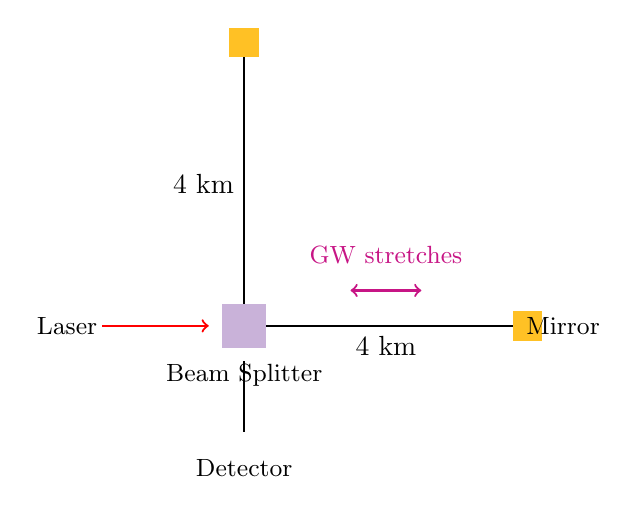
\begin{tikzpicture}[scale=0.9]
        % Arms
        \draw[thick] (0,0) -- (4,0) node[midway, below] {4 km};
        \draw[thick] (0,0) -- (0,4) node[midway, left] {4 km};

        % Beam splitter
        \filldraw[cosmicpurple!30] (-0.3,-0.3) rectangle (0.3,0.3);
        \node at (0,-0.7) {\small Beam Splitter};

        % Mirrors
        \filldraw[stargold] (3.8,-0.2) rectangle (4.2,0.2);
        \filldraw[stargold] (-0.2,3.8) rectangle (0.2,4.2);
        \node at (4.5,0) {\small Mirror};

        % Laser
        \draw[->, thick, red] (-2,0) -- (-0.5,0);
        \node at (-2.5,0) {\small Laser};

        % Detector
        \draw[thick] (0,-0.5) -- (0,-1.5);
        \node at (0,-2) {\small Detector};

        % GW effect
        \draw[<->, nebulapink, thick] (1.5,0.5) -- (2.5,0.5);
        \node[nebulapink] at (2,1) {\small GW stretches};
    \end{tikzpicture}
    \caption{Simplified LIGO interferometer schematic. Gravitational waves stretch one arm while compressing the other.}
    \label{fig:ligo}
\end{figure}

\subsection{Major Detections}

\begin{table}[H]
\centering
\caption{Notable gravitational wave detections.}
\label{tab:gw_events}
\begin{tabular}{|l|l|l|l|}
\hline
\textbf{Event} & \textbf{Date} & \textbf{Source} & \textbf{Significance} \\
\hline
GW150914 & Sep 2015 & 36+29 $\msun$ BBH merger & First detection \\
GW170817 & Aug 2017 & 1.4+1.4 $\msun$ BNS merger & First with EM counterpart \\
GW190521 & May 2019 & 85+66 $\msun$ BBH merger & Intermediate mass BH formed \\
\hline
\end{tabular}
\end{table}

\subsection{Multi-Messenger Astronomy}

GW170817 (neutron star merger) was observed in:
\begin{itemize}[noitemsep]
    \item Gravitational waves (LIGO/Virgo)
    \item Gamma rays (Fermi, INTEGRAL) --- 1.7 seconds after merger
    \item Optical/infrared ``kilonova'' --- hours to weeks
    \item Radio afterglow --- months later
\end{itemize}

This confirmed that neutron star mergers produce heavy elements (gold, platinum, uranium) through r-process nucleosynthesis.

\begin{funfactbox}
All the gold on Earth---every wedding ring, every Olympic medal---was forged in the violent collision of neutron stars billions of years ago, then scattered through space and incorporated into our solar system's formation.
\end{funfactbox}

\newpage

% ============================================
% SECTION 8: GALAXY CLUSTERS
% ============================================
\section{Galaxy Clusters: Cosmic Laboratories}
\label{sec:clusters}

\lettrine[lines=3, loversize=0.1, nindent=0.5em]{G}{alaxy} clusters are the largest gravitationally bound structures in the universe, containing hundreds to thousands of galaxies, vast amounts of hot gas, and enormous dark matter halos.

\subsection{Cluster Composition}

\begin{table}[H]
\centering
\caption{Typical galaxy cluster composition.}
\label{tab:cluster_composition}
\begin{tabular}{|l|c|l|}
\hline
\textbf{Component} & \textbf{Mass Fraction} & \textbf{Detection Method} \\
\hline
Dark Matter & 80--85\% & Gravitational lensing, dynamics \\
Intracluster Medium (ICM) & 12--15\% & X-ray emission \\
Galaxies (stars) & 3--5\% & Optical/infrared \\
\hline
\end{tabular}
\end{table}

\subsection{X-ray Observations}

Hot intracluster gas ($T \sim 10^7$--$10^8$ K) emits X-rays through thermal bremsstrahlung:

\begin{equationbox}
\begin{equation}
L_X \propto n_e^2 \sqrt{T} \cdot V
\end{equation}
\end{equationbox}

\begin{figure}[H]
    \centering
    \begin{minipage}{0.48\textwidth}
        \centering
        \includegraphics[width=\textwidth]{../images/scientific/perseus_cluster_xray.png}
        \caption{Chandra X-ray image of Perseus Cluster showing sound waves rippling through the hot gas.}
        \label{fig:perseus}
    \end{minipage}\hfill
    \begin{minipage}{0.48\textwidth}
        \centering
        \includegraphics[width=\textwidth]{../images/scientific/chandra_galaxy_clusters.png}
        \caption{Compilation of galaxy clusters observed by Chandra X-ray Observatory.}
        \label{fig:chandra_clusters}
    \end{minipage}
\end{figure}

\subsection{The Perseus Cluster Sound Waves}

In 2003, Chandra discovered pressure waves in the Perseus Cluster gas---essentially sound waves generated by the central black hole's jets:

\begin{itemize}[noitemsep]
    \item Wavelength: $\sim 30$ kpc
    \item Period: $\sim 10$ million years
    \item Frequency: $3 \times 10^{-15}$ Hz
    \item Musical note: B-flat, 57 octaves below middle C
\end{itemize}

\subsection{Cluster Classification}

\begin{itemize}[noitemsep]
    \item \textbf{Relaxed/Cool-Core ($\sim$70\%):} Symmetric, central temperature drop, AGN feedback (e.g., Perseus, Virgo)
    \item \textbf{Disturbed/Merging ($\sim$30\%):} Asymmetric, shock fronts, ongoing collision (e.g., Bullet Cluster)
    \item \textbf{Fossil Groups:} Single dominant elliptical galaxy---the merger remnant
\end{itemize}

\newpage

% ============================================
% SECTION 9: DEEP FIELD OBSERVATIONS
% ============================================
\section{Deep Field Observations}
\label{sec:deepfield}

\subsection{Hubble Ultra Deep Field}

The Hubble Ultra Deep Field (HUDF) represents one of the deepest images of the universe ever taken:

\begin{figure}[H]
    \centering
    \includegraphics[width=0.75\textwidth]{../images/scientific/hubble_ultra_deep_field.png}
    \caption{Hubble Ultra Deep Field---approximately 10,000 galaxies in an area smaller than a grain of sand held at arm's length.}
    \label{fig:hudf}
\end{figure}

\begin{table}[H]
\centering
\caption{Hubble Ultra Deep Field observation parameters.}
\label{tab:hudf}
\begin{tabular}{|l|l|}
\hline
\textbf{Parameter} & \textbf{Value} \\
\hline
Location & Fornax constellation \\
Angular size & 11 arcmin$^2$ (1/13 millionth of sky) \\
Total exposure & 1 million seconds (11.3 days) \\
Galaxy count & $\sim 10,000$ \\
Redshift range & $z = 0$ to $z \sim 12$ \\
Lookback time & 0 to 13.2 billion years \\
\hline
\end{tabular}
\end{table}

\textbf{Extrapolation:} If the HUDF is representative, the observable universe contains approximately $2 \times 10^{11}$ galaxies.

\newpage

% ============================================
% SECTION 10: OBSERVATIONAL INSTRUMENTS
% ============================================
\section{Observational Instruments \& Techniques}
\label{sec:instruments}

\subsection{Space-Based Telescopes}

\begin{table}[H]
\centering
\caption{Major space-based astronomical observatories.}
\label{tab:space_telescopes}
\small
\begin{tabular}{|l|l|l|l|l|}
\hline
\textbf{Telescope} & \textbf{Wavelength} & \textbf{Mirror} & \textbf{Launch} & \textbf{Key Discoveries} \\
\hline
Hubble & Optical/UV/IR & 2.4 m & 1990 & Deep fields, dark energy \\
Chandra & X-ray & Grazing incidence & 1999 & Cluster gas, BH jets \\
Spitzer & Infrared & 0.85 m & 2003 & Exoplanets, distant galaxies \\
Planck & Microwave & 1.5 m & 2009 & CMB precision cosmology \\
JWST & Infrared & 6.5 m & 2021 & First galaxies, exoatmospheres \\
Euclid & Optical/NIR & 1.2 m & 2023 & Dark energy, weak lensing \\
\hline
\end{tabular}
\end{table}

\subsection{Ground-Based Facilities}

\begin{table}[H]
\centering
\caption{Major ground-based observatories.}
\label{tab:ground_telescopes}
\small
\begin{tabular}{|l|l|l|l|}
\hline
\textbf{Facility} & \textbf{Type} & \textbf{Location} & \textbf{Capability} \\
\hline
VLT & Optical (4$\times$8.2m) & Chile & Interferometry, AO \\
Keck & Optical (2$\times$10m) & Hawaii & Spectroscopy \\
ALMA & Radio (66 dishes) & Chile & Sub-mm, $z>6$ galaxies \\
EHT & Radio VLBI & Global & $\mu$as resolution \\
LIGO/Virgo & Gravitational wave & USA/Italy & $h \sim 10^{-23}$ \\
\hline
\end{tabular}
\end{table}

\subsection{Future Missions}
Upcoming: \textbf{Vera Rubin Observatory} (2025, 8.4m survey), \textbf{Nancy Grace Roman} (2027, infrared), \textbf{LISA} (2037, space GW), \textbf{ELT} (2028, 39m mirror).

\newpage

% ============================================
% SECTION 11: SCIENTIFIC IMAGE GALLERY
% ============================================
\section{Scientific Image Gallery}
\label{sec:gallery}

\begin{figure}[H]
    \centering
    \begin{minipage}{0.48\textwidth}
        \centering
        \includegraphics[width=\textwidth]{../images/scientific/dark_matter_infographic.png}
        \caption{Universe's mass-energy content.}
        \label{fig:dm_infographic}
    \end{minipage}\hfill
    \begin{minipage}{0.48\textwidth}
        \centering
        \includegraphics[width=\textwidth]{../images/scientific/collision_diagram_dark.png}
        \caption{Galaxy cluster collision dynamics.}
        \label{fig:collision}
    \end{minipage}
\end{figure}

\begin{figure}[H]
    \centering
    \includegraphics[width=0.65\textwidth]{../images/extras/skys-the-limit-big-bang.jpg}
    \caption{Artistic visualization of cosmic expansion from the Big Bang.}
    \label{fig:bigbang_art}
\end{figure}

\newpage

% ============================================
% SECTION 12: PROJECT POSTER & TEAM
% ============================================
\section{Project Poster \& Team}
\label{sec:team}

\subsection{The Physical Poster}

Our project includes a large-format printed poster summarizing the key concepts of dark matter, black holes, and the Big Bang theory. The poster was designed for educational display and public outreach.

\begin{figure}[H]
    \centering
    \includegraphics[width=0.85\textwidth]{../images/poster-image.jpg}
    \caption{The Invisible Universe project poster showcasing dark matter, black holes, and Big Bang cosmology.}
    \label{fig:poster}
\end{figure}

\subsection{Team BomBSquad}

This project was developed collaboratively by Team BomBSquad, with each member contributing to specific areas of research and presentation.

\begin{figure}[H]
    \centering
    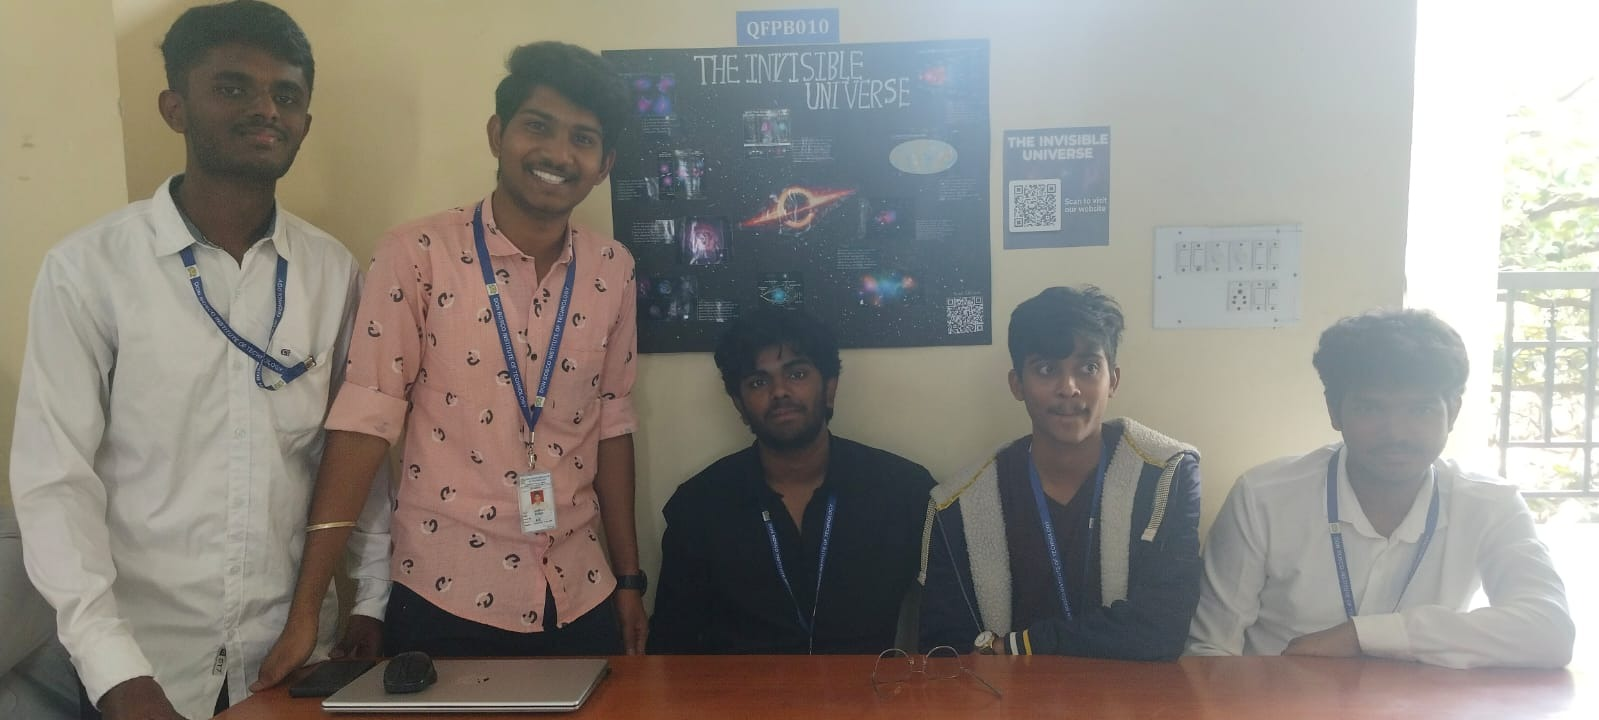
\includegraphics[width=0.85\textwidth]{../images/poster-imagewithteammates.png}
    \caption{Team BomBSquad members with the project poster.}
    \label{fig:poster_team}
\end{figure}

\begin{table}[H]
\centering
\caption{Team BomBSquad member contributions.}
\label{tab:contributions}
\begin{tabular}{|l|c|l|}
\hline
\textbf{Name} & \textbf{Roll No.} & \textbf{Primary Contribution} \\
\hline
Harsha N & 25B007 & Dark Matter Research \& Analysis \\
Hemanth Kumar KP & 25B013 & Black Hole Physics \& Visualization \\
Mithun Gowda B & 25B051 & Big Bang Theory \& Timeline \\
Naren V & 25B055 & Website Development \& Report Writing \\
Nevil Anson Dsouza & 25B058 & Poster Design \& Video Production \\
\hline
\end{tabular}
\end{table}

\subsection{Project Deliverables}

\begin{enumerate}[noitemsep]
    \item \textbf{Physical Poster:} Large-format printed display summarizing dark matter, black holes, and Big Bang cosmology
    \item \textbf{Interactive Website:} \url{https://narenvk-29.github.io/Invisible-Universe/}
    \item \textbf{Documentary Video:} 5-minute narrated presentation exploring the invisible universe
    \item \textbf{PDF Presentation:} Visual summary with key scientific imagery
    \item \textbf{Comprehensive Report:} This technical document with detailed explanations
\end{enumerate}

\newpage

% ============================================
% SECTION 13: CONCLUSION
% ============================================
\section{Conclusion}
\label{sec:conclusion}

\subsection{Summary of Findings}

This comprehensive investigation has explored the invisible universe through three fundamental pillars, each revealing profound insights about the nature and structure of the cosmos. Furthermore, the interconnections between these phenomena demonstrate how dark matter, black holes, and the Big Bang are intimately linked in the grand tapestry of cosmic evolution:

\begin{itemize}[noitemsep]
    \item \textbf{Dark Matter:} Multiple independent observations confirm that $\sim$85\% of all matter is non-luminous and non-baryonic ($\Omega_{DM} = 0.259$). Evidence includes galaxy rotation curves, cluster dynamics, gravitational lensing, the Bullet Cluster, and CMB anisotropies.

    \item \textbf{Black Holes:} Once theoretical curiosities, now directly observed via the Event Horizon Telescope (M87*, Sgr A*) and gravitational waves (LIGO/Virgo with 90+ detections). These observations confirm general relativity in extreme gravity regimes.

    \item \textbf{Big Bang Cosmology:} The universe originated 13.8 billion years ago from an initial hot, dense state. Evidence includes the CMB (2.725 K blackbody), primordial element abundances, Hubble expansion, and large-scale structure evolution.
\end{itemize}

Additionally, dark energy, which constitutes approximately 68\% of the universe, drives the accelerating cosmic expansion with an equation of state parameter $w \approx -1$, thereby representing one of physics' greatest mysteries.

\subsection{Open Questions \& Future Prospects}

Notwithstanding our remarkable progress, several fundamental mysteries remain unanswered: What is the true nature of dark matter? What physical mechanism causes dark energy? What, if anything, existed before the Big Bang? Consequently, the next decade promises transformative observational capabilities that may finally address these profound questions. Specifically, LISA will detect gravitational waves from supermassive black hole mergers, CMB-S4 will search for primordial gravitational waves from inflation, and the combined power of JWST, Euclid, and Roman will map cosmic evolution with unprecedented precision. Moreover, ground-based experiments continue to push the boundaries of dark matter detection sensitivity, while theoretical advances in quantum gravity may eventually illuminate the earliest moments of cosmic history.

\begin{center}
\begin{tcolorbox}[colback=lightcosmic, colframe=cosmicpurple, width=0.85\textwidth, arc=3mm]
    \centering
    \textit{``We are a way for the cosmos to know itself.''} --- Carl Sagan
\end{tcolorbox}
\end{center}

\newpage

% ============================================
% GLOSSARY
% ============================================
\section{Glossary of Terms}
\label{sec:glossary}

\begin{multicols}{2}
\footnotesize
\textbf{Axion:} Light dark matter candidate. \textbf{Baryon:} Protons, neutrons. \textbf{Big Bang:} Universe origin model. \textbf{Black Hole:} Gravity traps light. \textbf{CMB:} Cosmic Microwave Background. \textbf{Dark Energy:} Accelerating expansion (68\%). \textbf{Dark Matter:} Invisible matter (27\%). \textbf{Event Horizon:} Black hole boundary. \textbf{Friedmann Eq.:} Expansion equations. \textbf{Gravitational Lensing:} Light bending by mass. \textbf{Gravitational Waves:} Spacetime ripples. \textbf{Hawking Radiation:} BH thermal emission. \textbf{Hubble Constant:} $H_0 \approx 67$ km/s/Mpc. \textbf{ICM:} Cluster hot gas. \textbf{Inflation:} Early rapid expansion. \textbf{Kerr Metric:} Rotating BH solution. \textbf{LIGO:} GW observatory. \textbf{Nucleosynthesis:} Element formation. \textbf{Planck Epoch:} $t < 10^{-43}$ s. \textbf{Recombination:} Atoms form (380,000 yr). \textbf{Redshift:} Wavelength stretching. \textbf{Schwarzschild Radius:} $r_s = 2GM/c^2$. \textbf{Type Ia SN:} Standard candle. \textbf{WIMP:} Dark matter candidate.
\end{multicols}

\newpage

% ============================================
% REFERENCES
% ============================================
\section{References}
\label{sec:references}

\subsection{Foundational Scientific Papers}
\small
\begin{enumerate}[noitemsep]
    \item Zwicky, F. (1933). ``Die Rotverschiebung von extragalaktischen Nebeln.'' \textit{Helvetica Physica Acta}, 6, 110-127. [First dark matter proposal from galaxy cluster dynamics]
    \item Rubin, V. C. \& Ford, W. K. (1970). ``Rotation of the Andromeda Nebula from a Spectroscopic Survey of Emission Regions.'' \textit{The Astrophysical Journal}, 159, 379-403. [Galaxy rotation curves evidence]
    \item Penzias, A. A. \& Wilson, R. W. (1965). ``A Measurement of Excess Antenna Temperature at 4080 Mc/s.'' \textit{The Astrophysical Journal}, 142, 419-421. [CMB discovery - Nobel Prize 1978]
    \item Riess, A. G., et al. (1998). ``Observational Evidence from Supernovae for an Accelerating Universe and a Cosmological Constant.'' \textit{The Astronomical Journal}, 116, 1009-1038. [Dark energy discovery - Nobel Prize 2011]
    \item Perlmutter, S., et al. (1999). ``Measurements of Omega and Lambda from 42 High-Redshift Supernovae.'' \textit{The Astrophysical Journal}, 517, 565-586. [Independent dark energy confirmation]
    \item Clowe, D., et al. (2006). ``A Direct Empirical Proof of the Existence of Dark Matter.'' \textit{The Astrophysical Journal Letters}, 648, L109-L113. [Bullet Cluster evidence]
    \item EHT Collaboration (2019). ``First M87 Event Horizon Telescope Results. I. The Shadow of the Supermassive Black Hole.'' \textit{The Astrophysical Journal Letters}, 875, L1. [First black hole image]
    \item Abbott, B. P., et al. (2016). ``Observation of Gravitational Waves from a Binary Black Hole Merger.'' \textit{Physical Review Letters}, 116, 061102. [First gravitational wave detection - Nobel Prize 2017]
    \item Planck Collaboration (2020). ``Planck 2018 results. VI. Cosmological parameters.'' \textit{Astronomy \& Astrophysics}, 641, A6. [Precision cosmology measurements]
    \item Hawking, S. W. (1974). ``Black hole explosions?'' \textit{Nature}, 248, 30-31. [Hawking radiation theory]
    \item Schwarzschild, K. (1916). ``Über das Gravitationsfeld eines Massenpunktes nach der Einsteinschen Theorie.'' \textit{Sitzungsberichte der Königlich Preussischen Akademie der Wissenschaften}, 189-196. [First black hole solution]
    \item Einstein, A. (1915). ``Die Feldgleichungen der Gravitation.'' \textit{Sitzungsberichte der Preussischen Akademie der Wissenschaften}, 844-847. [General relativity field equations]
    \item Hubble, E. (1929). ``A Relation between Distance and Radial Velocity among Extra-Galactic Nebulae.'' \textit{Proceedings of the National Academy of Sciences}, 15, 168-173. [Universe expansion discovery]
    \item Gamow, G. (1948). ``The Evolution of the Universe.'' \textit{Nature}, 162, 680-682. [Big Bang nucleosynthesis]
    \item Guth, A. H. (1981). ``Inflationary universe: A possible solution to the horizon and flatness problems.'' \textit{Physical Review D}, 23, 347-356. [Cosmic inflation theory]
\end{enumerate}

\subsection{Books and Textbooks}
\begin{enumerate}[noitemsep]
    \item Weinberg, S. (1972). \textit{Gravitation and Cosmology: Principles and Applications of the General Theory of Relativity}. Wiley. [Comprehensive GR textbook]
    \item Hawking, S. W. (1988). \textit{A Brief History of Time}. Bantam Books. [Popular science classic]
    \item Carroll, S. (2004). \textit{Spacetime and Geometry: An Introduction to General Relativity}. Addison-Wesley. [Modern GR textbook]
    \item Ryden, B. (2017). \textit{Introduction to Cosmology}. Cambridge University Press. [Standard cosmology text]
    \item Kolb, E. W. \& Turner, M. S. (1990). \textit{The Early Universe}. Addison-Wesley. [Early universe physics]
    \item Thorne, K. S. (1994). \textit{Black Holes and Time Warps: Einstein's Outrageous Legacy}. W.W. Norton. [Black hole physics for general readers]
    \item Greene, B. (1999). \textit{The Elegant Universe}. W.W. Norton. [String theory and beyond]
    \item Tyson, N. D. \& Goldsmith, D. (2004). \textit{Origins: Fourteen Billion Years of Cosmic Evolution}. W.W. Norton.
\end{enumerate}

\subsection{Online Resources and Databases}
\begin{itemize}[noitemsep]
    \item NASA Science: \url{https://science.nasa.gov/} --- Official NASA science portal
    \item Hubble Space Telescope: \url{https://science.nasa.gov/mission/hubble/} --- Images and discoveries
    \item Event Horizon Telescope: \url{https://eventhorizontelescope.org/} --- Black hole imaging
    \item LIGO Scientific Collaboration: \url{https://www.ligo.org/} --- Gravitational wave detection
    \item James Webb Space Telescope: \url{https://science.nasa.gov/mission/webb/} --- Next-generation observations
    \item Chandra X-ray Observatory: \url{https://chandra.harvard.edu/} --- X-ray astronomy
    \item ESA/Hubble: \url{https://esahubble.org/} --- European Space Agency resources
    \item arXiv.org: \url{https://arxiv.org/archive/astro-ph} --- Preprint server for astrophysics
    \item NASA/IPAC Extragalactic Database: \url{https://ned.ipac.caltech.edu/} --- Galaxy data
    \item SIMBAD Astronomical Database: \url{https://simbad.u-strasbg.fr/} --- Astronomical objects
    \item Sloan Digital Sky Survey: \url{https://www.sdss.org/} --- Large-scale sky survey
    \item European Southern Observatory: \url{https://www.eso.org/} --- Ground-based astronomy
\end{itemize}

\subsection{Recent Research (2024--2025)}
\begin{enumerate}[noitemsep]
    \item Particle Data Group (2024). ``Review of Particle Physics: Dark Matter.'' \textit{Physical Review D}, 110, 030001. [Comprehensive dark matter review --- 26.4\% of cosmic density]
    \item EHT Collaboration (2024). ``First Sagittarius A* Event Horizon Telescope Results. VII. Polarization of the Ring.'' \textit{The Astrophysical Journal Letters}. [Magnetic fields around Sgr A*]
    \item EHT Collaboration (2024). ``First Sagittarius A* Event Horizon Telescope Results. VIII. Physical Interpretation of the Polarized Ring.'' \textit{The Astrophysical Journal Letters}.
    \item Raymond, A.W., Doeleman, S., et al. (2024). ``First Very Long Baseline Interferometry Detections at 870 $\mu$m.'' \textit{The Astronomical Journal}. [Highest-resolution black hole detection]
    \item Baczko, A.-K., et al. (2024). ``The putative center in NGC 1052.'' \textit{Astronomy \& Astrophysics}. [Black hole jet imaging]
    \item LIGO-Virgo-KAGRA Collaboration (2024). ``GW230529: Observation of a Neutron Star-Mass Gap Compact Object Merger.'' [Mass gap detection]
    \item LIGO-Virgo-KAGRA (2025). ``GWTC-4.0: Updated Gravitational-Wave Catalog.'' \textit{The Astrophysical Journal Letters}. [250+ merger events from O4]
    \item Bertone, G., Hooper, D., \& Silk, J. (2005). ``Particle dark matter: evidence, candidates and constraints.'' \textit{Physics Reports}, 405, 279-390. [Major dark matter review --- 5000+ citations]
    \item Gupta, R. P. (2024). ``Testing CCC+TL Cosmology with Observed Baryon Acoustic Oscillation Features.'' \textit{The Astrophysical Journal}, 964(1), 55. [Alternative cosmological model]
\end{enumerate}

\subsection{Educational Videos and Documentaries}
\begin{itemize}[noitemsep]
    \item \textit{Cosmos: A Spacetime Odyssey} (2014) --- Neil deGrasse Tyson, National Geographic
    \item \textit{Black Holes: The Edge of All We Know} (2020) --- Documentary on EHT project
    \item \textit{The Universe} (History Channel series) --- Comprehensive astronomy coverage
    \item PBS Space Time (YouTube) --- Advanced physics explanations
    \item Veritasium, Kurzgesagt --- Science communication channels
\end{itemize}

\subsection{Data Archives and Catalogs}
\begin{itemize}[noitemsep]
    \item GWTC (Gravitational-Wave Transient Catalog): \url{https://gwosc.org/} --- 250+ detected events
    \item Planck Legacy Archive: \url{https://pla.esac.esa.int/} --- CMB data and maps
    \item Dark Energy Survey: \url{https://www.darkenergysurvey.org/} --- Galaxy survey data
    \item Gaia Archive: \url{https://gea.esac.esa.int/} --- Stellar positions and motions
\end{itemize}

\vfill

\begin{center}
\rule{0.7\textwidth}{0.4pt}\\[0.3cm]
{\Large\bfseries Team BomBSquad}\\[0.2cm]
\textit{The Invisible Universe Project}\\[0.2cm]
\url{https://narenvk-29.github.io/Invisible-Universe/}\\[0.5cm]

\begin{tcolorbox}[colback=lightcosmic, colframe=cosmicpurple, width=0.8\textwidth, arc=3mm]
    \centering
    \textit{``Somewhere, something incredible is waiting to be known.''}\\[0.1cm]
    --- Carl Sagan
\end{tcolorbox}
\end{center}

\end{document}
